\documentclass[11pt]{article}
\usepackage{acl2010}
\usepackage{times}
\usepackage{url}
\usepackage{latexsym}
\usepackage{graphicx}
\usepackage{amsmath}
\usepackage{url}
\usepackage{multirow}
\usepackage{rotating}
%\setlength\titlebox{6.5cm}    
% You can expand the title box if you really have to


\DeclareMathOperator*{\argmax}{arg\,max}

\newcommand{\mnote}[1]{\marginpar{%
  \vskip-\baselineskip
  \raggedright\footnotesize
  \itshape\hrule\smallskip\footnotesize{#1}\par\smallskip\hrule}}  

\title{Learning Structural and Sentential Paraphrases from Parallel Corpora}

\author{Juri Ganitkevitch \and Chris Callison-Burch\\ 
Center for Language and Speech Processing\\ 
Johns Hopkins University}

\date{}

\begin{document}
\maketitle

\begin{abstract}
  \begin{itemize}
  \item ``in this work'' stuff is implied
  \item newcites rather than cites 
  \item put a little brag claim at the end, summarizing the outcome
  \item abstract should tell you whether paper is interesting, whether
    your results are interesting
  \item motivate the problem
  \item briefly motivate choices
  \item be clear, sell the paper to the reviewers
  \item be direct, motivate and explain instead of saying ``we
    motivate/explain''
  \item briefly tie back to previous work
  \item concrete numbers
  \end{itemize}
  Paraphrase extraction approaches based on richly annotated
  monolingual parallel corpora have been
\end{abstract}

\section{Introduction} \label{introduction}

Paraphrases are alternative ways to express the same meaning. The
automated generation and detection of paraphrases is crucial to many
tasks in NLP and has been shown to improve performance in others. In
multi-document summarization systems, paraphrase detection can be used
to recognize and collapse redundancies \cite{Barzilay1999}. Used for
query expansion, paraphrasing improves the performance of question
answering \cite{Ravichandran2002,Riezler2007} and information
retrieval systems \cite{Anick1999}. In statistical machine translation (SMT),
paraphrases have been used to extend phrase tables in order to achieve
broader source language coverage \cite{Callison-Burch2006b}, as well
as to automatically generate additional reference translations,
leading to better results in minimum error rate training
\cite{Madnani2007}.

The notion of a paraphrase typically denotes a set of surface text
forms with the same meaning:
\begin{center}
\begin{tabular}{c}
the committee's proposal \\
the proposal of the committee
\end{tabular}
\end{center}
Introducing non-terminals or \emph{slots}, lexical paraphrases are
commonly generalized into paraphrase patterns such as:
\begin{center}
\begin{tabular}{c}
the $X_1$'s $X_2$ \\
the $X_2$ of the $X_1$
\end{tabular}
\end{center}
It is evident that, compared to plain phrases, paraphrase patterns
have a much higher potential at generalization. However, the
unconstrained nature of the slots also bears the risk of producing
nonsensical or ungrammatical output. Thus, in order to achieve more
well-formed results, the slots are typically augmented with syntactic
constraints, yielding syntactic paraphrases.
\begin{center}
\begin{tabular}{c}
the $NP_1$'s $NP_2$ \\
the $NP_2$ of the $NP_1$
\end{tabular}
\end{center}
While retaining the generalization capabilities of unconstrained
patterns, the application of syntactic paraphrases is more controlled
and yields higher quality output.

\mnote{Sentential paraphrases, and all the transforms we want to
  learn. Unclear whether we can get them from bitexts.. ..let's find out.}

In this paper, we demonstrate the integration of syntactic paraphrases
into an SMT-based paraphrasing system. The use of SMT machinery and
models to extract and apply paraphrases from bilingual parallel
corpora by pivoting over foreign language phrases is a well-known
technique. \newcite{Zhao2008b} have presented results that indicate
that bilingually sourced paraphrase extraction significantly
outperforms monolingual approaches in both recall and
precision. However, while in monolingually sourced paraphrase
extraction linguistically informed paraphrase patterns are
commonplace, SMT-based paraphrase systems mostly have been limited to
lexical paraphrases \cite{Quirk2004,Callison-Burch2005} or
unconstrained patterns \cite{Madnani2007}. In recent efforts to enrich
pivot-based paraphrase extraction with linguistic information
\newcite{Callison-Burch2008} showed that enforcing syntactic
constraints can drastically improve the quality of a lexical
paraphrase system. \newcite{Zhao2008} used dependency parses on the
English side of a large bilingual corpus to produce syntactic
parapharse patterns. Our approach goes beyond these two and produces a
fully syntactically informed synchronous paraphrasing CFG.

An additional focus of this paper are the closely tied topics of model
parameter estimation and system evaluation. In practice, the nature of
paraphrasing as a component of larger systems makes meaningful
standalone evaluation difficult: in many applications of paraphrasing
the proper preservation of meaning and production of grammatical
output is only a basis requirement. Additional constraints imposed by
the task at hand, be it shortening the input for sentence compression
or generating significantly differing output for the generation of
additional references, are a crucially important factor for the
system's quality. However, this is often not reflected when estimating
the parameters of a paraphrasing system. We leverage the rich feature
set present in our approach and the flexibily of minimum error rate
training to specifically adapt our paraphrase system to the task of
reference expansion for SMT and demonstrate how it outperforms the
commonly used approach.

This paper is structured as follows: we present related work on
paraphrase acquisition in
Section~\ref{related_work}. Section~\ref{formalism} introduces the
machine translation model used in our work. In
Section~\ref{acquisition} we describe our paraphrase acquisition
approach. Sections~\ref{adaptation} and \ref{analysis} present our
parametere estimation setup, experimental and an analysis
thereof. Finally, we conclude in Section~\ref{conclusion}.

\section{Related Work} \label{related_work}

The paraphrase extraction task has received a fair amount of attention
in the past. In this paper we extend a method for extracting
paraphrases from bilingual parallel corpora that was introduced by
\newcite{Callison-Burch2005}. \newcite{Callison-Burch2005} generate
paraphrases using techniques from {\it phrase-based} statistical
machine translation \cite{Koehn2003}. After extracting a bilingual
phrase table, English paraphrases can be extracted by pivoting through
foreign language phrases. The phrase table contains phrase pairs $(e,
f)$ (where the $e$ and $f$ stand for English and foreign phrases,
respectively) as well as bi-directional translation probabilities
$p(f | e)$ and $p(e | f)$, computed from the relative frequencies of
$e$ and $f$. From this table, they compute a paraphrasing phrase table
with entries $(e, e')$. Since many paraphrases can be extracted for a
phrase, \newcite{Callison-Burch2005} define a paraphrase probability
to rank them:
% \begin{equation}
%   \hat{e_2} = \argmax_{e_2:e_2 \neq e_1} p(e_2|e_1)
% \end{equation}
% where
\begin{eqnarray}
  p(e_2|e_1) &=& \sum_f p(e_2,f|e_1)\\
                  &=& \sum_f p(e_2|f,e_1) p(f|e_1) \\
                  &\approx& \sum_f p(e_2|f) p(f|e_1)
\label{paraphrase_prob_eqn}
\end{eqnarray}
Additionally, the resulting paraphrases are further re-ranked using
contextual features such as a language model.
\newcite{Callison-Burch2008} improves on this method by requiring the
paraphrases to be governed by the same constituent, resulting in less
noisy and more grammatical paraphrases.

\newcite{Madnani2007} apply the pivot technique to {\it hierarchical}
phrase-based machine translation \cite{Chiang2005}. Hierarchical
phrases contain a variable ``X'' that allows for slot-fillers.
\newcite{Madnani2007}'s paraphrase table contains these slotted
patterns as well. Because hierarchical phrase-based machine
translation is formally a synchronous context free grammar (SCFG),
\newcite{Madnani2007}'s paraphrase table can be thought of as a {\it
  paraphrase grammar}. Their paraphrase grammar can paraphrase (or
``decode'') input sentences using an SCFG decoder, like the Hiero MT
system. \newcite{Madnani2007} mirror Hiero's log-linear model and its
feature set. The parameters for the log-linear model are estimated
using minimum error rate training, maximizing the BLEU metric on a set
of parallel English sentences. The authors report significant gains in
translation quality when using additional references generated by
paraphrasing to tune a machine translation system.

\newcite{Zhao2008} further enrich pivot-based paraphrase approach with
syntactic information by extracting partial subtrees from a
dependency-parsed English side of a bitext and pivoting over the
corresponding Chinese phrases to extract paraphrases. The slots in the
resulting patterns are labeled with part-of-speech tags (but not
larger syntactic constituents). Their system also employs a log-linear
model that combines translation and lexical probabilities and is tuned
to maximize precision over a hand-labeled set of paraphrases.

Several research efforts have leveraged parallel monolingual corpora,
however they jointly suffer from the scarcity and noisiness of
parallel corpora. \mnote{Ah, yes. That's some excellent English right
  there.} \newcite{Dolan2004} work around this issue by extracting
parallel sentences from the vast amount of freely available comparable
English text and apply machine translation techniques to create a
paraphrasing system \cite{Quirk2004}. However, the word-based
translation model and monotone decoder they use results in a
substantial amount of identity paraphrases or single-word
substitutions.

Relying on small data sets of semantically equivalent translations,
\newcite{Pang2003} created finite state automata by syntax-aligning
parallel sentences, enabling the generation of additional reference
translations.

Both \newcite{Barzilay2001} and \newcite{Ibrahim2003} sentence-align
existing noisy parallel monolingual corpora such as translations of
the same novels. While \newcite{Ibrahim2003} employ a set of
heuristics that rely on anchor words identified by textual identity or
matchin liguistic features such as gender, number or semantic class,
\newcite{Barzilay2001} use a co-training approach that leverages
context similarity to identify viable paraphrases.

Semantic parallelism is well-established as a stong basis for the
extraction of correspondencies such as paraphrases. However, there are
notable efforts that choose to forgo it in favor of clustering
approaches based on distributional characteristics. The well-known
DIRT method by \newcite{Lin2001} fully relies on distributional
similarity features for paraphrase extraction. Patterns extracted from
paths in dependency graphs are clustered based on the similarity of
the observed contents of their slots.

Similarly, \newcite{Bhagat2008} argue that vast amounts of text can be
leveraged to make up for the relative weakness of distributional
features compared to parallelism. They also forgo complex annotations
such as syntactic or dependency parses, relying only on part-of-speech
tags to inform their approach. In their work, relations are learned by
finding pattern clusters initially seeded by already known
patterns. However, this method is not capable of producing syntactic
paraphrases. \mnote{Need better tie-in with the overall theme of structural
paraphrases.}


\section{SCFGs in Translation} \label{formalism}

Similar to \newcite{Madnani2007}, our paraphrasing system heavily
relies on established statistical machine translation
machinery. \mnote{Spin this towards the section title.} The model we
use in our approach is \emph{Syntax Augmented Machine Translation} or
\emph{SAMT} \cite{Zollmann2006}, which is based on the \emph{
  synchronous context-free grammar} (SCFG) formalism and allows for an
arbitrary number of non-terminals.

Formally, a PSCFG $\mathcal{G}$ is defined by specifying
\[
\mathcal{G} = \langle \mathcal{N}, \mathcal{T}_S, \mathcal{T}_T,
\mathcal{R}, S \rangle ,
\]
where $\mathcal{N}$ is a set of non-terminal symbols, $\mathcal{T}_S$
and $\mathcal{T}_T$ are the source and target language vocabularies,
$\mathcal{R}$ is a set of rules and $S \in \mathcal{N}$ is the root
symbol. The rules in $\mathcal{R}$ take the form
\begin{equation*}
  C \rightarrow \langle \gamma, \alpha, \sim, w \rangle ,
\end{equation*}
where the rule's left-hand side $C \in \mathcal{N}$ is a non-terminal,
$\gamma \in (\mathcal{N} \cup \mathcal{T}_S)^*$ and $\alpha \in
(\mathcal{N} \cup \mathcal{T}_T)^*$ are strings of terminal and
non-terminal symbols with an equal number of non-terminals
$c_{\mathit{NT}}(\gamma) = c_{\mathit{NT}}(\alpha)$ and 
$$
\sim : \{1 \ldots c_{\mathit{NT}}(\gamma)\} \rightarrow \{1 \ldots
c_{\mathit{NT}}(\alpha)\}
$$ 
constitutes a one-to-one correspondency function between the
non-terminals in $\gamma$ and $\alpha$. A non-negative weight $w \geq
0$ is assigned to each rule, reflecting the likelihood of the rule.

\begin{figure*}[t]
\begin{center}
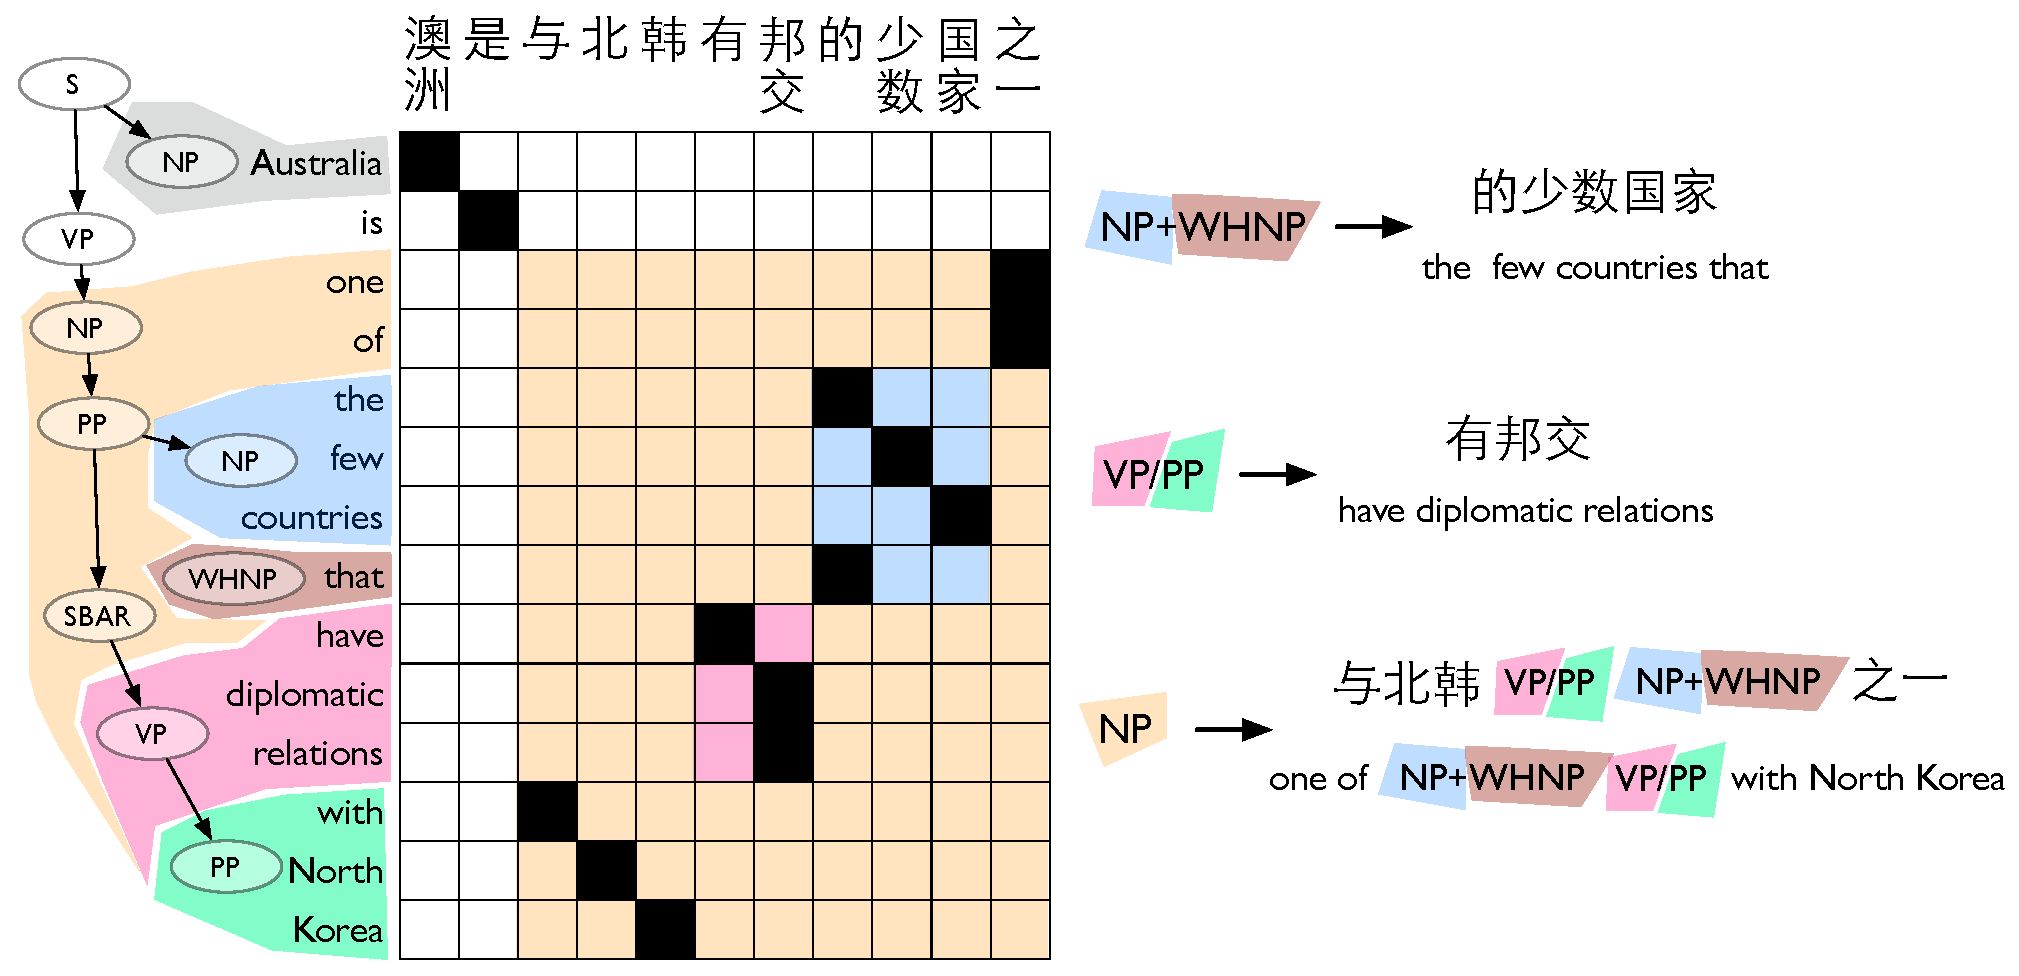
\includegraphics[width=0.99\linewidth]{figures/scfg_grid_revamp.pdf}
\end{center}
\caption{Make this prettier later on.}
\label{samt_extraction}
\end{figure*}

The rule set for an SAMT grammar is extracted from word-aligned
sentence-parallel corpora where the target language side is annotated
with syntactic parses. Figure~\ref{samt_extraction} shows an example
of rules obtained for one phrase pair. To extract a rule, we first
choose a target span $t$. The left-hand side of the rule is then given
by the syntactic constituent governing $t$. In addition to single
constituent non-terminals, SAMT allows for the concatenation of
constituents as well as for CCG-style non-terminal labels
\cite{Steedman1999}, which increases the grammar's coverage by
allowing for non-syntactic phases in the grammar. The source side of
the rule, $s$, is obtained by projecting $t$ over the word
alignment. To introduce non-terminals into the rule's source and
target sides, we can apply rules extracted over sub-phrases of $t$,
synchronously substituting the corresponding non-terminal symbol for
the sub-phrases on both sides. \mnote{Tie this back to $\alpha$ and
  $\gamma$?} The synchronous substitution applied to $t$ and $s$
yields the correspondency $\sim$.

Rather than assigning a weight $w$, SAMT stores a number of feature
values $\varphi_i$ for each rule, which are combined in a log-linear
model:
\begin{equation}
  w = \sum_i^N \lambda_i \varphi_i .
\end{equation}
For ease of notation, we will refer to $\varphi_1, \ldots ,\varphi_N$
as $\vec{\varphi}$. The feature set of the SAMT model by default
consists of 23 feature functions and covers a diverse set of rule
characteristics. We discuss our task-specific extensions to the SAMT
feature set in Section~\ref{adaptation}.

\section{SCFGs in Paraphrasing} \label{acquisition}

\begin{figure*}[!t]
\begin{center}
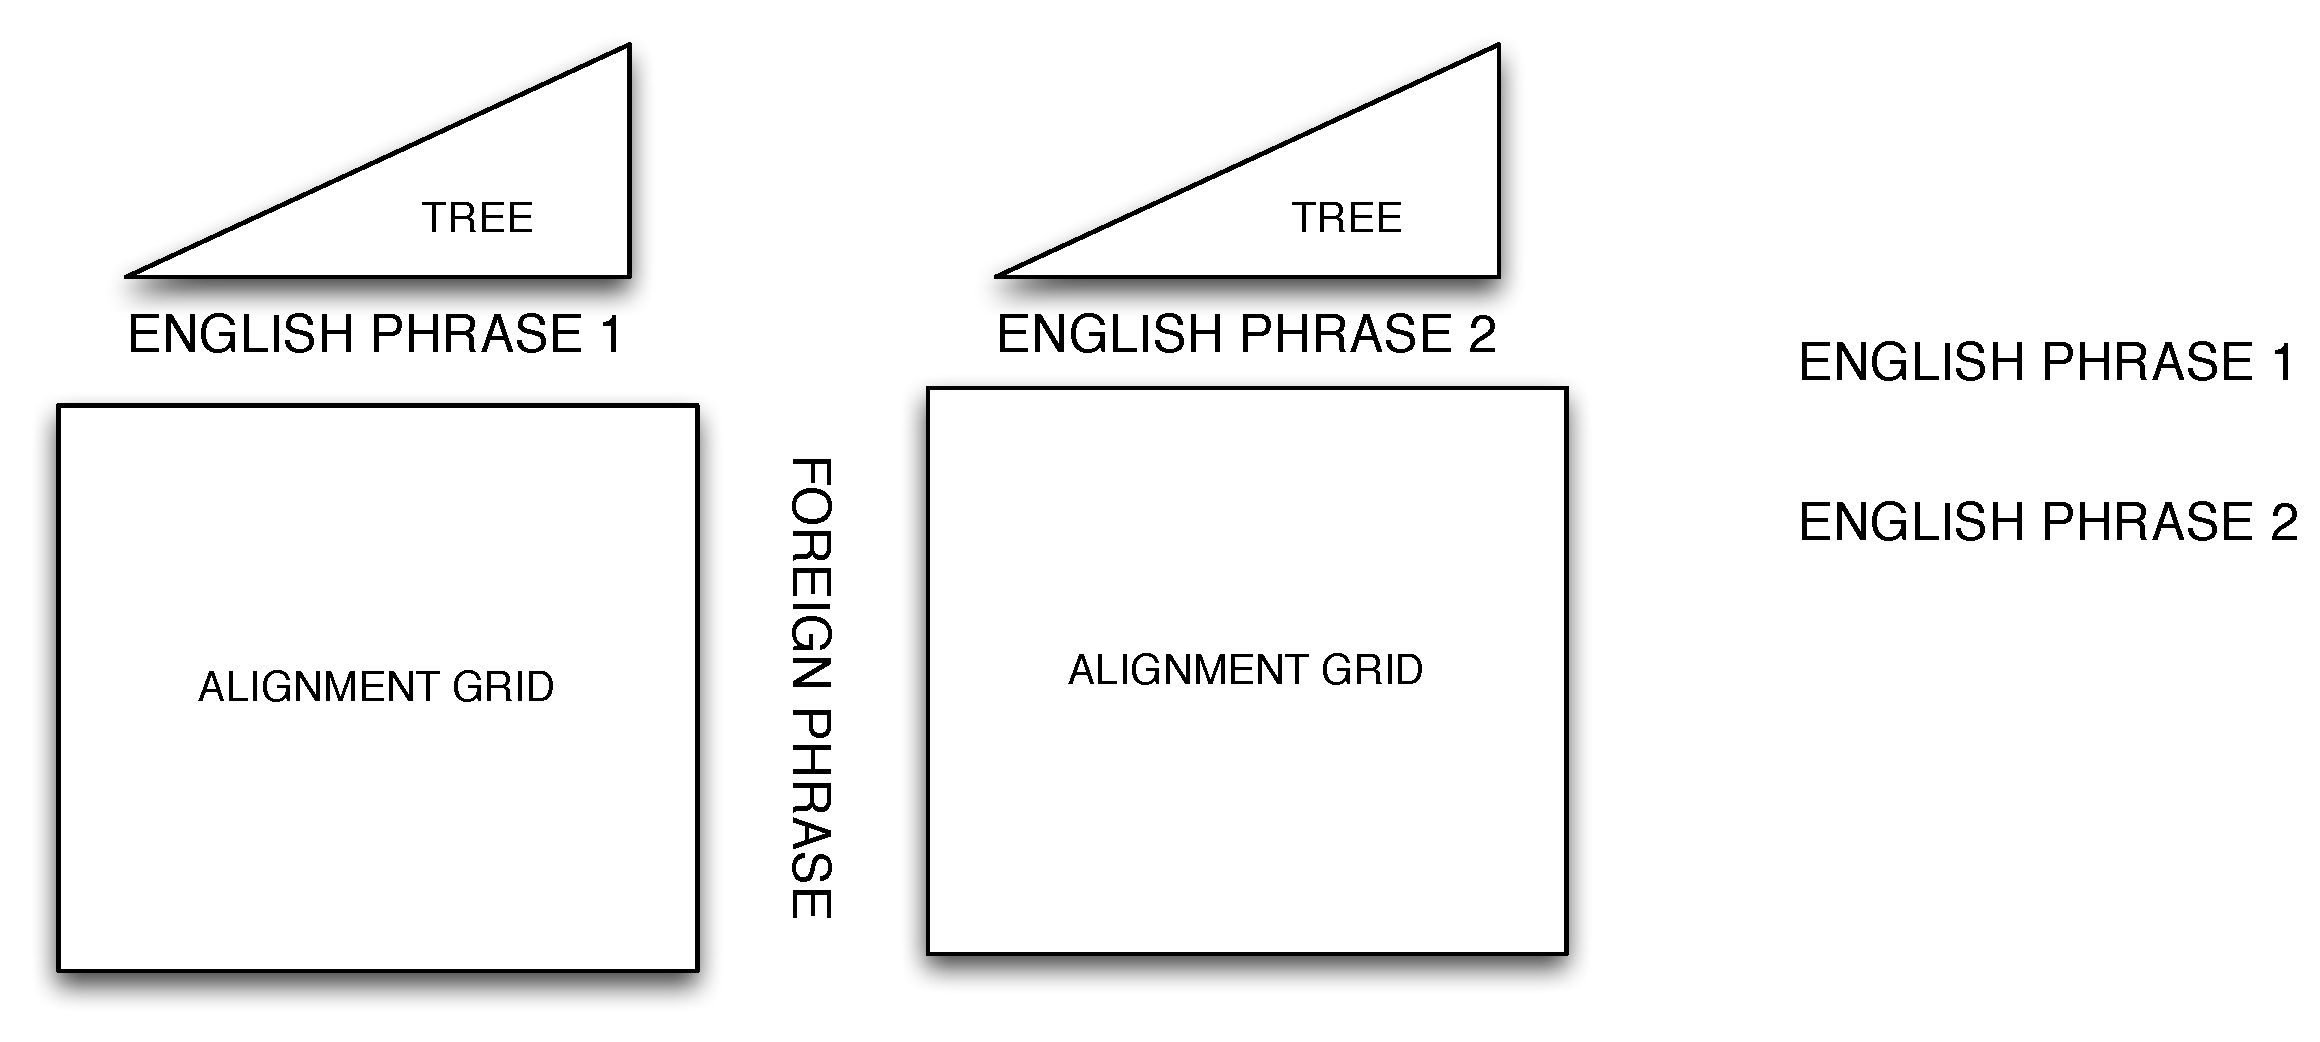
\includegraphics[width=0.99\linewidth]{figures/pivot.pdf}
\end{center}
\caption{Let's see if we need this}
\end{figure*}

To create a paraphrase grammar from a translation grammar, we extend
the pivot approach of \newcite{Callison-Burch2005} to the SAMT
model. For this purpose, we assume a grammar that translates from a
given foreign language to English. For each pair of translation rules where
the left-hand side $C$ and foreign string $\gamma$ match
\begin{eqnarray*}
C \rightarrow \langle \gamma, \alpha_1, \sim_1, \vec{\varphi}_1 \rangle \\
C \rightarrow \langle \gamma, \alpha_2, \sim_2, \vec{\varphi}_2 \rangle
\end{eqnarray*}
we create a paraphrase rule
\begin{equation*}
C \rightarrow \langle \alpha_1, \alpha_2, \sim, \vec{\varphi} \rangle ,
\end{equation*}
where the non-terminal correspondency relation $\sim$ has been set to
reflect the combined non-terminal alignment
\begin{equation*}
\sim ~ = ~ \sim_1^{-1} \circ \sim_2 .
\end{equation*}

\subsection{Feature Computation}

The computation of $\vec{\varphi}$ from $\vec{\varphi}_1$ and
$\vec{\varphi}_2$ occurs on feature level. For this purpose, the SAMT
feature set can be roughly partitioned into three groups.

The first group consists of features that depend solely on the rule
itself. This includes features based on number or nature of terminals
or non-terminals in $\alpha_1$ or $\alpha_2$, features that indicate
non-terminal reordering or deletion of punctuation and pseudo-features
like a glue rule indicator or the application count feature. Since
none of these features require additional information, their
computation for $\vec{\varphi}$ is straightforward.

The features in the second group additionally depend on aggregate
counts over the bitext and thus cannot be computed from the rule
alone. However, the information contained in $\vec{\varphi}_1$ and
$\vec{\varphi}_2$ allows us to apply the pivot approach as shown in
Equation~\ref{paraphrase_prob_eqn} to approxate the real feature value
for $\vec{\varphi}$. In the SAMT feature set, this group only includes
the four lexical translation probability features.

The remainder of the feature set falls into the third group. These
features depend on information that we cannot reconstruct from
$\vec{\varphi}_1$ and $\vec{\varphi}_2$. Features in this group
include the rule's probability conditioned on the left-hand-side, its
source side with and without non-terminal labels as well as rareness
and unbalancedness penalties. For these we fall back to a black-box
approach, treating the value for a given features as an indication of
the rule's quality in some particular aspect. To combine the feature
values, we multiply for the relative frequencies and add for the
penalty functions.

In addition to combining $\vec{\varphi}_1$ and $\vec{\varphi}_2$, we
extend $\vec{\varphi}$ by a paraphrasing-specific boolean feature
$\varphi_{\mathit{ident}}$, that is $1$ when $\alpha_1 = \alpha_2$ and
$0$ otherwise. This allows us to tune our system to prefer or
dis-prefer identity paraphrases.

\subsection{Grammar Pruning}

Due to the diverse set of non-terminals allowed in our model, the
grammars we extract tend to become extremely large. This, combined
with the multiplicative effect of pivoting, quickly makes the
resulting paraphrase grammars grow too large too handle.

To keep the grammars at a manageable size while retaining good
paraphrases, we implement a the following pruning approach. We only
consider translation rules that have been seen more than a given
number of times and exceed a given translation probability threshold
for pivot recombination. In addition to this, we rank the generated
paraphrases for each pattern according to a combination of translation
and lexical probablity and only retain the top $n$
alternatives. \mnote{This is a little wonky, maybe drop the top-$n$
  pruning?}

The result of this process is a paraphrase grammar with syntactic
annotations and a feature set which (approximately) mirrors that of
the initial translation grammar. We now move to estimating the
feature weights. \mnote{This is awful. Needs better intro into
  estimation part.}


\section{Analysis} \label{analysis}

When introducing syntactic information into our paraphrase extraction
model, a key aim is the acquisition of structural paraphrases. We
expect our training procedure to learn generalized, properly labeled
patterns that, ideally, will reflect well-know paraphrastic
transformations such as passivization, dative shift or the possessive
rule. Representing such transforms in a generic fashion, our
paraphrasing grammar would be capable of awesome things.

In examining a parpharse grammar obtained from a French-English
bitext, we find that this is indeed the
case. Table~\ref{example_rules} shows a selection of paraphrase rules
found in our grammar, labeled with the paraphrastic transformation the
effect.


\begin{table*}
  \begin{center}
  \begin{tabular}{|c|rrcl|}
    \hline
    Possessive rule & $\mathit{NP}$ $\rightarrow$  & the $\mathit{NNP}_1$'s
    $\mathit{NN}_2$ & $\mid$ & the $\mathit{NN}_2$ of the $\mathit{NNP}_1$
    \\

    Dative shift & $\mathit{VP}$ $\rightarrow$ & give $\mathit{NN}$ to
    $\mathit{NP}$ & $\mid$ & give $\mathit{NP}$ the $\mathit{NN}$ \\

    Passivization &
    $\mathit{SBAR}$ $\rightarrow$ & that $\mathit{NP}$ had
    $\mathit{VBN}$ & $\mid$ & which was $\mathit{VBN}$ by $\mathit{NP}$ \\

    Adverbial phrase move & 
    $\mathit{VP}$ $\rightarrow$ & $\mathit{VBN}$ $\mathit{ADVP}$ & $\mid$ & is
    $\mathit{ADVP}$ being $\mathit{VBN}$ \\

    Reduced relative clause & $\mathit{SBAR/S}$ $\rightarrow$ & in order
    to $\mathit{VB}$ that & $\mid$ & in order to $\mathit{VB}$ \\
    \hline
\end{tabular}
\end{center}
\caption{Examples of structural paraphrasing rules extracted by our
  system}
\label{example_rules}
\end{table*}

\subsection{Comparison of Paraphrase
  Patterns} \label{pattern_comparison}

To analyze the paraphrase patterns produced by our system, we reduce
the grammar to only patterns that apply to an example sentence and
take a closer look at the most likely pattern pairs. We contrast our
extracted paraphrases with a Hiero-style baseline that mirrors the
approach of \newcite{Madnani2007}. 

\begin{table*}[t]
\begin{center}
\begin{tabular}{|c|c|rrcl|}
  \hline
  Input phrase & \multicolumn{5}{c|}{Best extracted paraphrases} \\
  \hline
  \multirow{6}{*}{the dog's tail} &
  \multirow{3}{*}{H}
  &
  $\mathit{X}$ $\rightarrow$  & the $\mathit{X}_1$'s
  $\mathit{X}_2$ & $\mid$ & the $\mathit{X}_2$ of the $\mathit{X}_1$
  \\
  &&
  $\mathit{X}$ $\rightarrow$  & the $\mathit{X}_1$'s
  $\mathit{X}_2$ & $\mid$ & the $\mathit{X}_2$ of the $\mathit{X}_1$
  \\
  &&
  $\mathit{X}$ $\rightarrow$  & the $\mathit{X}_1$'s
  $\mathit{X}_2$ & $\mid$ & the $\mathit{X}_2$ of the $\mathit{X}_1$ \\
  \cline{2-6}
  & \multirow{3}{*}{S}
  &
  $\mathit{NP}$ $\rightarrow$  & the $\mathit{NNP}_1$'s
  $\mathit{NN}_2$ & $\mid$ & the $\mathit{NN}_2$ of the $\mathit{NNP}_1$
  \\
  &&
  $\mathit{NP}$ $\rightarrow$  & the $\mathit{NNP}_1$'s
  $\mathit{NN}_2$ & $\mid$ & the $\mathit{NN}_2$ of the $\mathit{NNP}_1$
  \\
  &&
  $\mathit{NP}$ $\rightarrow$  & the $\mathit{NNP}_1$'s
  $\mathit{NN}_2$ & $\mid$ & the $\mathit{NN}_2$ of the
  $\mathit{NNP}_1$ \\
  \hline
  \multirow{6}{*}{the dog's tail} &
  \multirow{3}{*}{H}
  &
  $\mathit{X}$ $\rightarrow$  & the $\mathit{X}_1$'s
  $\mathit{X}_2$ & $\mid$ & the $\mathit{X}_2$ of the $\mathit{X}_1$
  \\
  &&
  $\mathit{X}$ $\rightarrow$  & the $\mathit{X}_1$'s
  $\mathit{X}_2$ & $\mid$ & the $\mathit{X}_2$ of the $\mathit{X}_1$  \\
  &&
  $\mathit{X}$ $\rightarrow$  & the $\mathit{X}_1$'s
  $\mathit{X}_2$ & $\mid$ & the $\mathit{X}_2$ of the $\mathit{X}_1$
  \\
  \cline{2-6}
  & \multirow{3}{*}{S}
  &
  $\mathit{NP}$ $\rightarrow$  & the $\mathit{NNP}_1$'s
  $\mathit{NN}_2$ & $\mid$ & the $\mathit{NN}_2$ of the $\mathit{NNP}_1$
  \\
  &&
  $\mathit{NP}$ $\rightarrow$  & the $\mathit{NNP}_1$'s
  $\mathit{NN}_2$ & $\mid$ & the $\mathit{NN}_2$ of the $\mathit{NNP}_1$
  \\
  &&
  $\mathit{NP}$ $\rightarrow$  & the $\mathit{NNP}_1$'s
  $\mathit{NN}_2$ & $\mid$ & the $\mathit{NN}_2$ of the
  $\mathit{NNP}_1$ \\
  \hline
\end{tabular}
\end{center}
\caption{This table shows the top paraphrase rules matching an input
  phrase as ranked by our (S) and the baseline system (H).}
\end{table*}


\subsection{Sentential Paraphrasing} \label{sentential_paraphrasing}

We are interested in sentential paraphrases. Why are we interested?
More powerful than locally constrained, gives us large-scale changes
to sentential structure, which can be cruicial to applications such as
detecting entailment or automatically creating significantly differing
references. \emph{However, phrasal decoder-based approaches should be
  able to achieve similar re-ordering effects (if not the generality,
  which we only implicitely achieve, really). Maybe we should add a
  phrase-based baseline in addition to Hiero? Did Nitin talk about
  this?}

While the definition of a phrasal paraphrase is intuitively clear,
sentential paraphrases are much harder to define. When paraphrasing a
sentence $s$ into a new sentence $t$, the term suggests that we expect
the changes to $s$ to be above a certain threshold for $t$ to be
considered a sentential paraphrase.


\section{Parameter Estimation} 
\label{adaptation}

need to estimate parameters for both, paraphrase ranking and paraphrasing

since we use  mert

like nitin, we tune on ref-to-ref translation

however BLEU is bad, leads to identity paraphrases


We estimate the parameters of our log-linear model using minimum error
rate training \cite{Och2003}.

\subsection{Paraphrase BLEU} \label{pp_bleu}

The familiar BLEU metric \cite{Papineni2002} quantifies the quality of
a translation by measuring the n-gram overlap between the generated
translation and a set of reference translation

\begin{table}
\begin{center}
\begin{tabular}{|c|c|c|}
  \hline
  & BLEU & ppBLEU \\
  \hline
  Identity & good & bad \\
  Oracle & good & good \\
  \hline
\end{tabular}
\end{center}
\caption{Oracle experiment with references: ``translate'' ref onto
  itself score; ``translate'' ref onto heldout ref, score}
\end{table}

for paraphrasing, this can be a problem, since the reference
translations typically have a rather high overlap with one another
\mnote{get some numbers to back that up} and the decoder has to beat
that first


\section{Reference Expansion}

We present an examplary application of our paraphrasing system

Using paraphrases for reference expansion, cite Madnani

idea behind reference expansion: create additional ``reference''
translations to tune a machine translation system

however, tuning our paraphrase system to BLEU results in a paraphraser
that generates only minimal changes \mnote{if so, how did Madnani deal
with that?}

We therefore implement a paraphrase-specific metric, ppBLEU, that aims
to amend this issue.


\subsection{Data} \label{data}

We use Europarl v. 5. Align with Berkeley and parse with The Parser.

we use the SAMT pipeline to extract the grammar

however, the pivoting approach makes it impossible to apply the common pre-emptive
grammar filtering, hence the grammar grows very large

\subsection{Evaluation} \label{evaluation}

A straightforward way to evaluate a paraphrasing system is by using to
improve an SMT system's performance. Cite Chris and Nitin. Compare to
Hiero baseline



\section{Conclusion} \label{conclusion}

Look, we unified everything in the field and made all this stuff from
the previous section much better. Or did we?

\bibliographystyle{acl}
\bibliography{paraphrasing}

\nocite{*}

\end{document}

